%%%%%%%%%%%%%%%% Springer %%%%%%%%%%%%%%%%%%%%%%%%%%%%%%%%%%


\documentclass{svproc}
%
% RECOMMENDED %%%%%%%%%%%%%%%%%%%%%%%%%%%%%%%%%%%%%%%%%%%%%%%%%%%
%
\newtheorem{df}{Definition}
\usepackage{amsmath}
\usepackage{array}

\usepackage{color}
\usepackage{graphicx}

\usepackage[numbers,square,sort&compress]{natbib}
\bibliographystyle{spmpsci_unsrt}

% to typeset URLs, URIs, and DOIs
\usepackage{url}
\def\UrlFont{\rmfamily}

\begin{document}
\mainmatter              % start of a contribution
%
\title{Long term temperature data analysis for damage detection in electric motor bearings with density modeling and Bhattacharyya distance}
%
\titlerunning{Temperature analysis with density modeling}  % abbreviated title (for running head)
%                                     also used for the TOC unless
%                                     \toctitle is used
%Wiesław Migdał, Maciej Wuczyński, Jacek Wodecki, Agnieszka Wyłomańska, Radosław Zimroz
 \author{%
Wies{\l}aw Migda{\l}\inst{1}, Jacek Wodecki\inst{2}, Maciej Wuczy{\'n}ski\inst{2}, Pawe{\l} Stefaniak\inst{2},  Agnieszka Wy{\l}oma{\'n}ska\inst{2},  Rados{\l}aw Zimroz\inst{3}
}%
%
 \authorrunning{Wies{\l}aw Migda{\l} et al.} % abbreviated author list (for running head)
%
%%%% list of authors for the TOC (use if author list has to be modified)
% \tocauthor{Ivar Ekeland, Roger Temam, Jeffrey Dean, David Grove,
% Craig Chambers, Kim B. Bruce, and Elisa Bertino}
%


\institute{ 
UNICO Ltd Industrial Informatics Systems, Czerwi{\'n}skiego Str 6, 40-123 Katowice, Poland \\ \email{wmigdal@unico.com.pl} \and  
Research and Development Centre, KGHM Cuprum Ltd, Sikorskiego 2-8, 53-659 Wroclaw, Poland \\ \email{\{jwodecki, mwuczynski, pkstefaniak, awylomanska\}@cuprum.wroc.pl} \and  
Faculty of Geoengineering, Mining and Geology, Diagnostics and Vibro-Acoustic Science Laboratory, Wroclaw University of Science and Technology, Na Grobli 15, 50-421 Wroclaw, Poland\\ \email{radoslaw.zimroz@pwr.wroc.pl}
}

\maketitle              % typeset the title of the contribution

\begin{abstract}
In the paper we will show specific case study related to long-term temperature data from electric motor bearings (with progressing fault) used in belt conveyor operating in open-cast mine. Existing SCADA system for data acquisition has built-in simple decision making rules based on static thresholds. Due to time-varying environmental and operational conditions, i.e. machine is heavily influenced by ambient temperature (-20 up to +30 deg. Celsius) and external load (no operation, idle mode, startup with heavily overloaded belt). Hence, basic analytical methods based on simple statistics are sometimes not sufficient to determine the change of technical condition of the bearing. In order to address this issue authors propose an analytical method based on multidimensional distribution analysis. Finally, a clustering method can be applied to multidimensional representation of the initial data. This approach allows to differentiate the technical condition across the investigated time period.
\keywords{condition monitoring, Bhattacharyya distance, temperature data, statistical analysis}
\end{abstract}
\section{Introduction}

In polish open-cast mines belt conveyors play key role in generating productivity of the entire horizontal transportation system. They are designed to operate in the entire spectrum of difficult environmental conditions including various types of precipitation, broad range of ambient temperatures etc. To be able to maintain the conveyors in best technical condition possible, extensive monitoring systems are installed. Although amount of collected data is often very large, those systems are still lacking specialized analytical procedures required to obtain high-level diagnostic information.

In presented article authors are focusing on the subject of long-term condition monitoring of electric motor operating in driving station of belt conveyor using temperature from a rolling bearing \cite{wodecki2016condition,kruczek2017fault,wodecki2017technical}. This type of problem has been investigated by researchers in various fields, very often for wind turbines, automotive industry etc. \cite{sawicki2015automatic,yang2013data,guo2012wind,astolfi2014fault,yang2013wind,nembhard2013fault,crossman2003automotive,mana2017wind}. It is known that the bearing experienced a failure, after which temperature value began to increase far above typical ranges. Authors propose to treat individual days as portions of data and investigate the variation of value distribution \cite{wylomanska2015analysis}. In order to achieve that, kernel distribution estimator is used, and the feature of dissimilarity is defined as Bhattacharyya distance between consecutive distributions and pre-established model.

\subsection{Object of interest}

The effectiveness of the presented methodology will be demonstrated on the example of long-term observation of the temperature of the rolling bearing of an electric motor operating in the drive station of a belt conveyor in opencast mining industry. 

\begin{figure}[ht!]
\centering
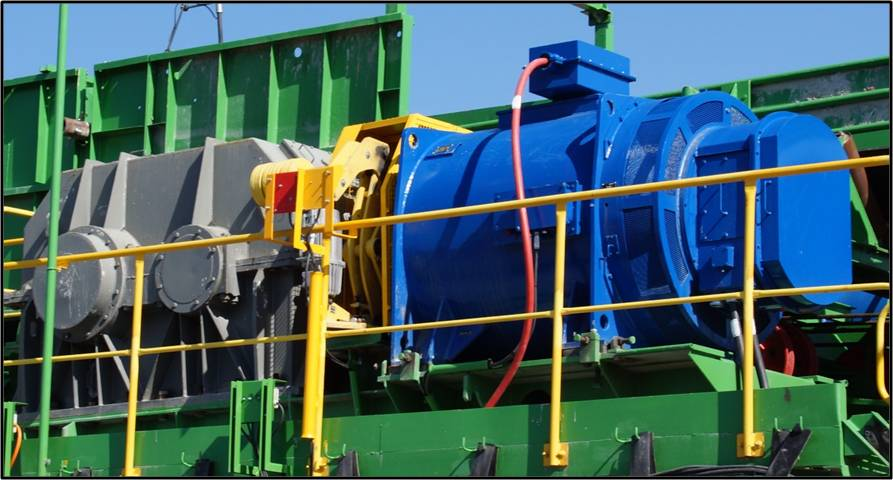
\includegraphics[width=0.9\textwidth]{figs/fig01.jpg}
\caption{An example view of an electric motor operating in the drive station of a belt conveyor}
\label{fig:block}
\end{figure}

Electric motors used in drive stations of belt conveyors working in opencast mining are usually devices with high nominal electrical powers, supplied with three-phase electrical voltage of value mainly 6 [kV]. The subject motor, whose all measurable parameters were observed in the long term, had the specification presented in Table \ref{tab:tab2}.

\begin{table}[ht!]
    \centering
    \caption{Parameters of considered engine}
    \begin{tabular}{|l|l|}
    \hline
         Construction & asynchronous annular three-phase motor  \\ \hline
         Power & 1,000 [kW] \\ \hline
         Voltage & 6 [kV] \\ \hline
         Current & 98 [A] \\
    \hline
    \end{tabular}
    \label{tab:tab2}
\end{table}

The motor is started using a four-stage resistance starter as a function of time. The start-up process is fully automated. Measured parameters after processing into digital signals are transferred via transmission networks to the Data Warehouse. Data collected in the Data Warehouse where analytical algorithms are implemented, are subject to the process of contextual analysis. The results of the analyzes are used by the maintenance services, but also by the crew responsible for managing the production costs. 


\section{Methodology}

\begin{figure}[ht!]
\centering
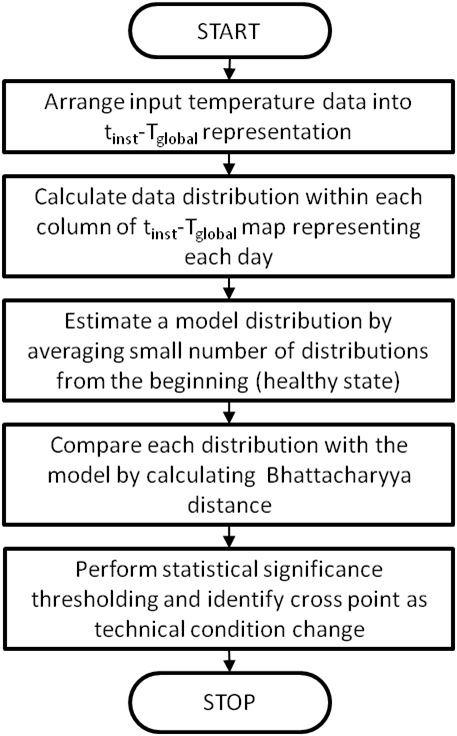
\includegraphics[width=0.6\textwidth]{figs/fig02.png}
\caption{Flowchart of presented procedure}
\label{fig:block}
\end{figure}

In this section authors present details of described method (see Fig. \ref{fig:block}). In the first step long-term temperature signal is rearranged to form time-time representation. It is constructed in the form of two-dimensional real-valued matrix in such a way that columns represent consecutive days of recorded data and are recognized as \emph{global time $T_{global}$}, and single column contains temperature record for a single day, which is called \emph{local time $t_{inst}$}. In this context one can understand this representation as a function of two different time dimensions $Temp=f(t_{inst},T_{global})$.

After constructing such two-dimensional map, distribution density for each day is modeled using kernel density estimator. Such operation produces density map that can be described as a function of global time $T_{global}$ (on horizontal axis) and temperature values $Temp$ (as a domain of density distribution, on vertical axis), in short $D=f(Temp,T_{global})$. 

In the next step model distribution is estimated by averaging small number of distributions from the beginning of the entire signal, where machine is known to operate in healthy state. Then every column of density map is compared to the model by calculating Bhattacharyya distance. Distance vector constructed that way is normalized and thresholded with standard statistical significance level $l=5\%$. First value to cross that threshold is identified as the beginning of a day of damage occurrence. Obviously precision of presented methodology is limited to a single day, because this is the length of density estimation window.

\begin{figure}[ht!]
\centering
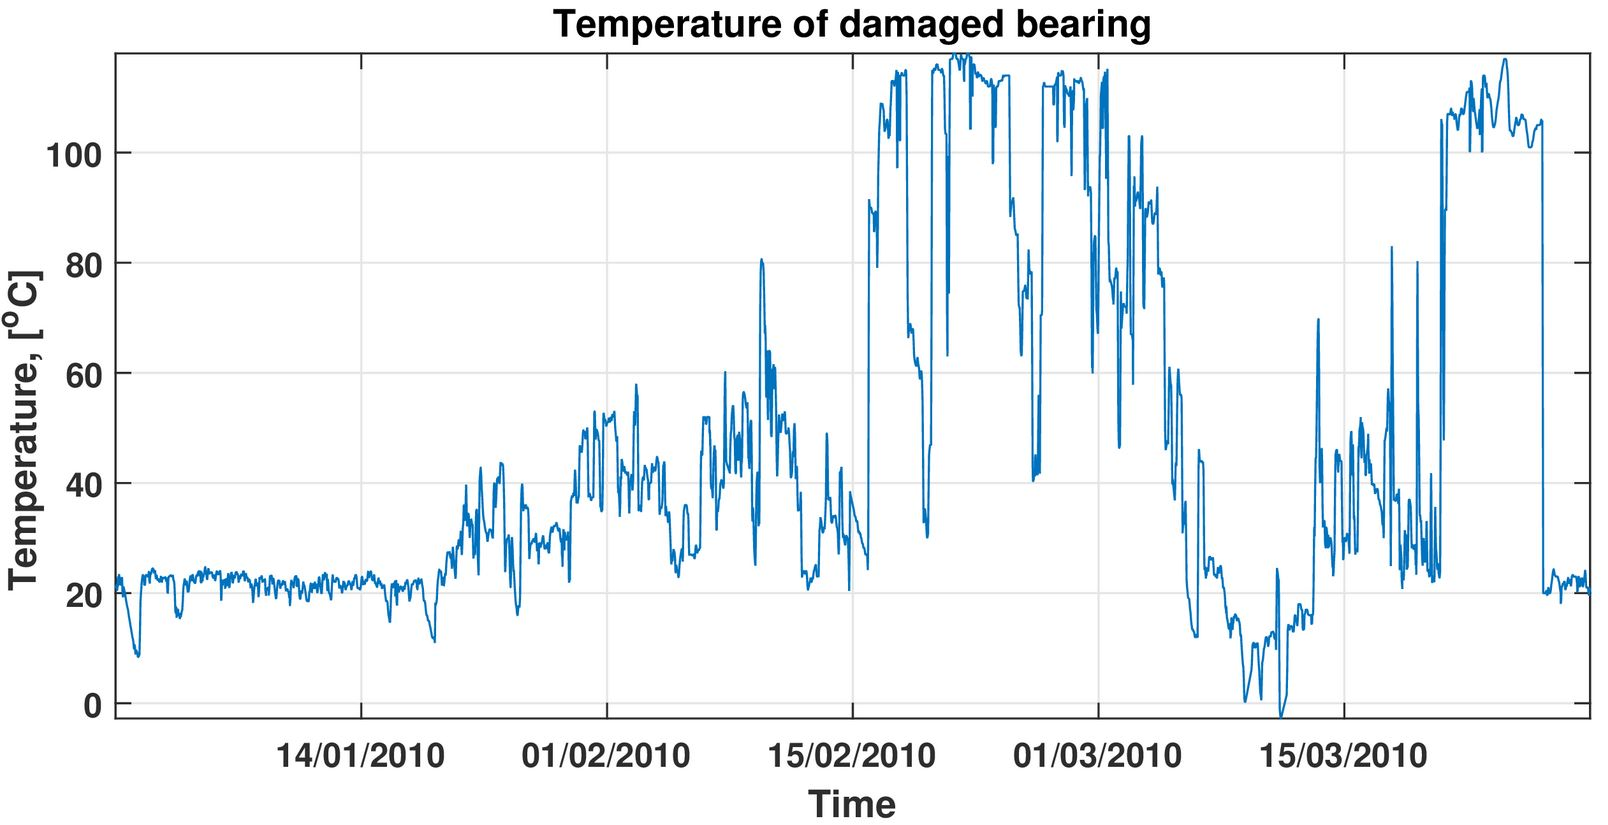
\includegraphics[width=\textwidth]{figs/Fig03.jpg}
\vspace*{-15pt}
\caption{Input temperature data}
\vspace*{-10pt}
\label{fig:raw}
\end{figure}

\subsection{Density distribution estimation}

In presented application density distribution is estimated using kernel density estimator, which is the estimated probability density function of a random variable \cite{peter1985kernel,silverman1986density}. For any real values of $x$, the kernel density estimator's formula is given by:

\begin{equation*}
    \hat{f}_h(x)=\frac{1}{nh} \sum_{i=1}^{n}K\left( \frac{x-x_i}{h}\right),
\end{equation*}
where $x_1, x_2, \dots , x_n$ are random samples from an unknown distribution, $n$ is the sample size, $\mathbf{K(\cdot)}$ is the kernel smoothing function, and $h$ is the bandwidth. In this implementation standard Gaussian kernel is used.

The value of bandwidth is obtained using so-called \emph{Silverman's rule of thumb} \cite{silverman1986density}. If Gaussian basis functions are used to approximate univariate data, and the underlying density being estimated is Gaussian, the optimal choice for $h$ (that is, the bandwidth that minimizes the mean integrated squared error) is:

\begin{equation*}
    h=\left( \frac{4\hat{\sigma}^5}{3n} \right)^{\frac{1}{5}} \approx 1.06\hat{\sigma}n^{-1/5},
\end{equation*}
where $\hat{\sigma}$ is the standard deviation of the samples and $n$ is number of samples.

\begin{figure}[ht!]
\centering
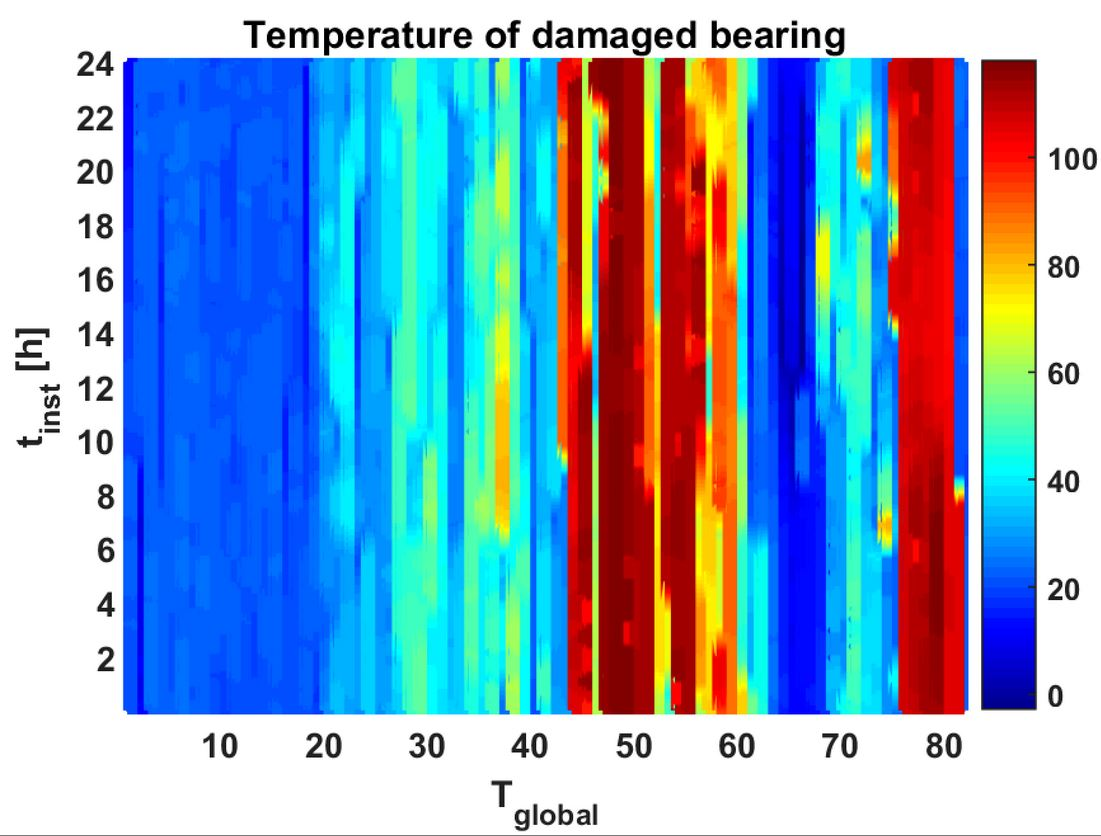
\includegraphics[width=0.9\textwidth]{figs/Fig04.jpg}
\caption{Described representation matrix. Columns indicate consecutive days, rows are timestamps within a day}
\label{fig:map1}
\end{figure}

\subsection{Bhattacharyya distance}

In statistics, the Bhattacharyya distance measures the similarity of two discrete or continuous probability distributions, named after Anil Kumar Bhattacharya, Indian statistician who worked in the 1930s. The Bhattacharyya distance is widely used in research of feature extraction and selection \cite{choi2003feature}.

For probability distributions described by density functions $p$ and $q$ over the same domain \textbf{X}, the Bhattacharyya distance is defined as:

\begin{equation*}
    D_B(p,q)=-ln(BC(p,q)),
\end{equation*}
where

\begin{equation*}
    BC(p,q)=\sum_{x \in X} \sqrt{p(x)q(x)}
\end{equation*}
is the Bhattacharyya coefficient for discrete probability distributions.

\begin{figure}[ht!]
\centering
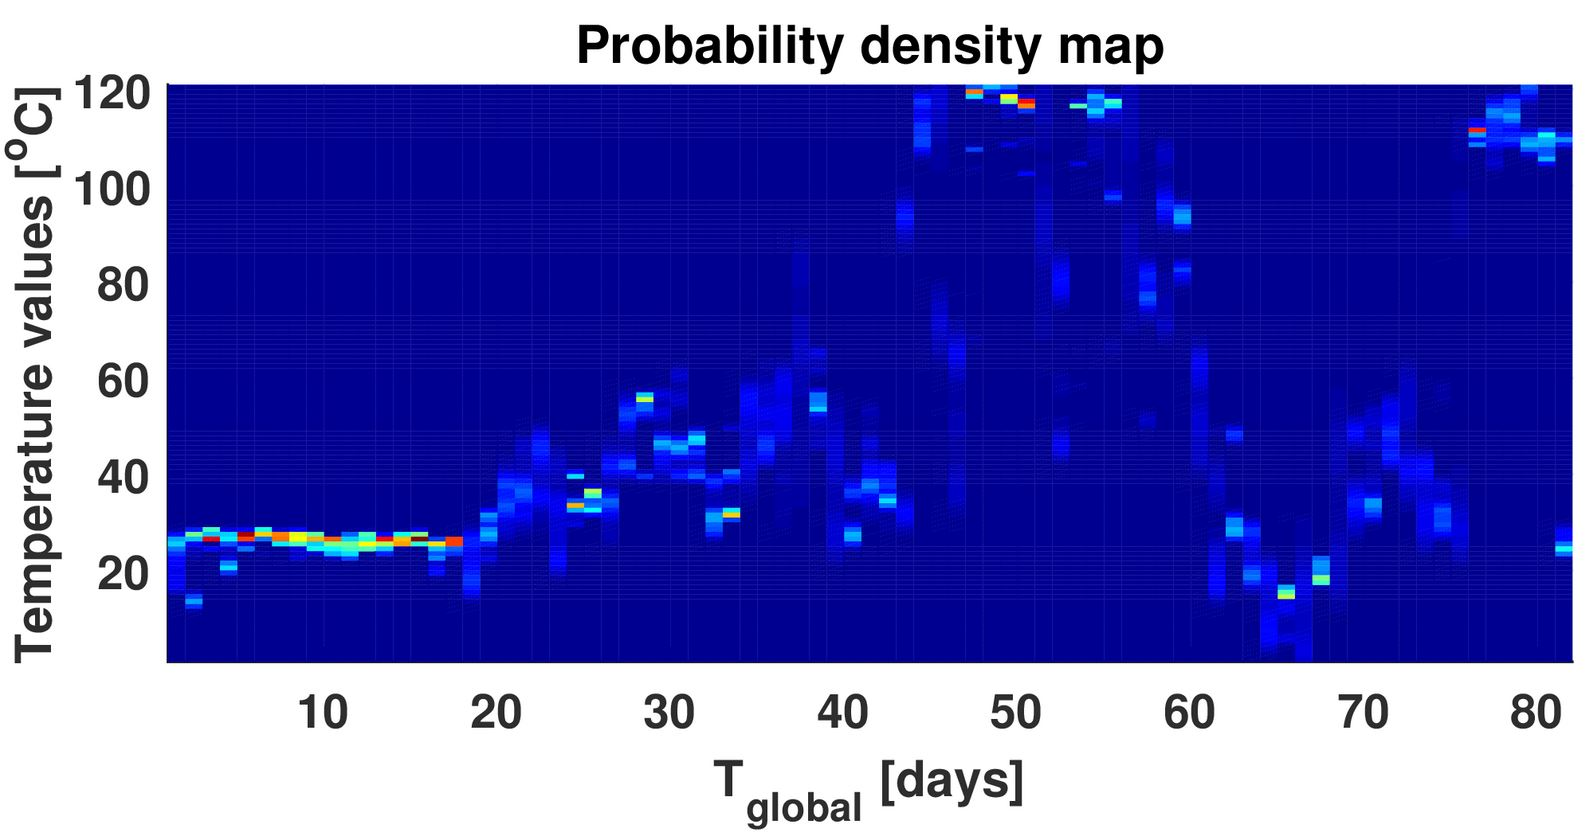
\includegraphics[width=0.9\textwidth]{figs/Fig05.jpg}
\caption{Distribution density map}
\label{fig:map2}
\end{figure}

\section{Results}\label{res}

In the first step raw input data (see Fig. \ref{fig:raw}) have been transformed to $t_{inst}-T_{global}$ representation presented in Fig. \ref{fig:map1}. After that distribution density has been estimated and distribution density map has been constructed (see Fig. \ref{fig:map2}).

\begin{figure}[ht!]
\centering
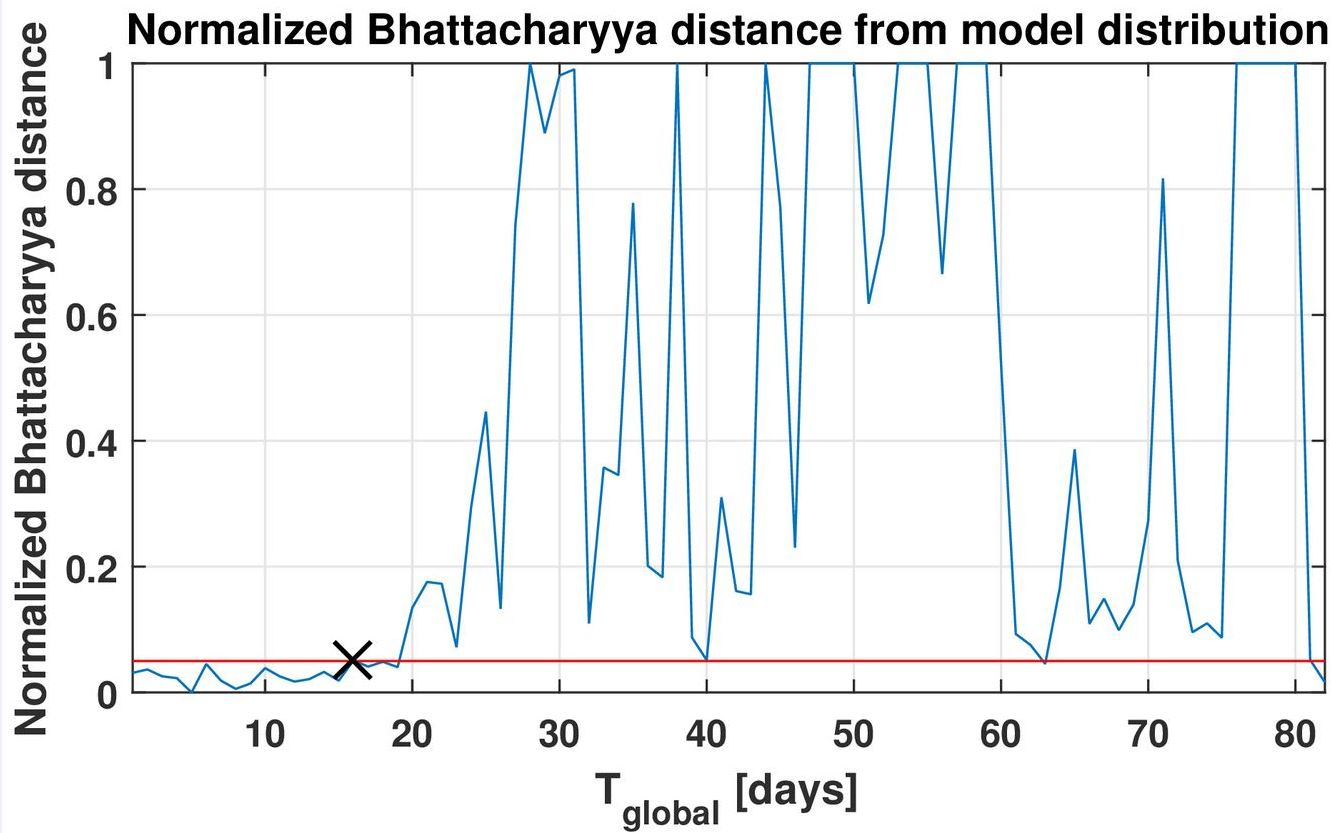
\includegraphics[width=\textwidth]{figs/Fig06.jpg}
\vspace*{-10pt}
\caption{Normalized Bhattacharyya distance as a feature vector for event detection. Black cross marks the localized moment of failure}
\label{fig:duty}
\end{figure}

After determining model distribution based on first five days (about $6\%$) of recorded data, it has been compared to every distribution vector in the density matrix, and Bhattacharyya distance was measured. Distance vector constructed from obtained values is presented in Fig. \ref{fig:duty}.

Finally, distance vector was normalized to the (0,1) range and statistical significance threshold was established at $5\%$. First distance value rising above the threshold is identified as the moment of failure occurrence.

\begin{figure}[ht!]
\centering
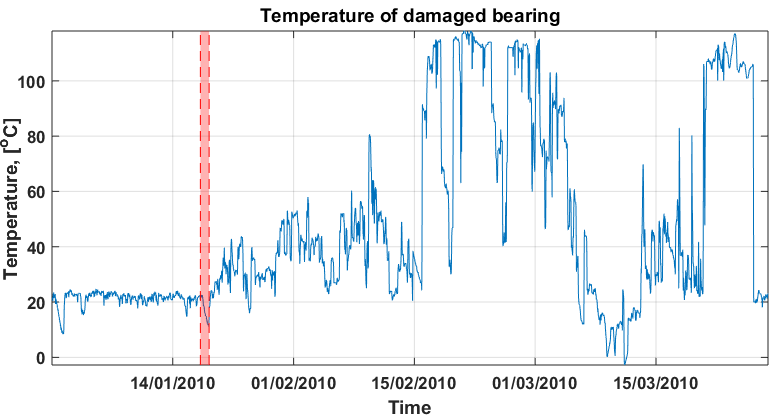
\includegraphics[width=\textwidth]{figs/fig07.png}
\caption{Results of analysis. Red area indicates the confidence boundary of failure occurrence}
\label{fig:out}
\end{figure}

Since the accuracy of presented method cannot be greater than a single day (due to global time resolution of density map) it is proposed to indicate the result as an area of confidence between the beginning and the end of detected day.

\section{Conclusions}

In this paper authors introduce an interesting approach to failure detection in the scenario of long-term record of a single diagnostic variable. Considered physical system was strongly time-varying, which was one of the main difficulties in correct identification of fault appearance in temperature data. To deal with such inconvenience in time domain, authors proposed method based on density distribution modeling of temperature data within consecutive days of operation. Statistical comparison of distribution functions allowed to identify moment of fault. Unfortunately at the current stage of development precision of the method is limited to one day, due to the way that temperature data is transformed to dual time representation. Hence, authors intend to improve the method in the future by developing more robust way to calculate distribution density functions from temperature data. This will allow to achieve much greater precision.

\bibliography{mybibfile}
\end{document}
